\section{Additional results}
\label{app:results}

\paragraph{The v1 model, re-evaluated.} The original GLWM paper reported a mean of 1.05 steps with a gate
initialised to halt early. Re-running it with the evaluation of this paper (deduplicated test set,
exact match over all positions, \cref{tab:v1}) shows that both initialisations reach full accuracy,
the v1 initialisation uses 2.6 steps on average, and only 84\% of instances are already correct after
one step (\cref{fig:v1}). The earlier step count came from a halting criterion that stopped before the
answer had settled.

\begin{table}[h]
  \centering
  \caption{The v1 GLWM model with a fixed gate initialisation versus the original (v1) initialisation,
  evaluated on the deduplicated 4--8 digit test set.}
  \label{tab:v1}
  \small
  \begin{tabular}{lrrrrr}
\toprule
Gate init & Accuracy & Mean steps & Steps (4-digit) & Acc.\ at step 1 & MFLOPs/sample \\
\midrule
fixed & 1.0000 $\pm$ 0.0000 & 3.41 & 3.87 & 0.5888 & 7.50 \\
v1 & 1.0000 $\pm$ 0.0000 & 2.60 & 3.05 & 0.8405 & 7.02 \\
\bottomrule
\end{tabular}
\end{table}

\begin{figure}[h]
  \centering
  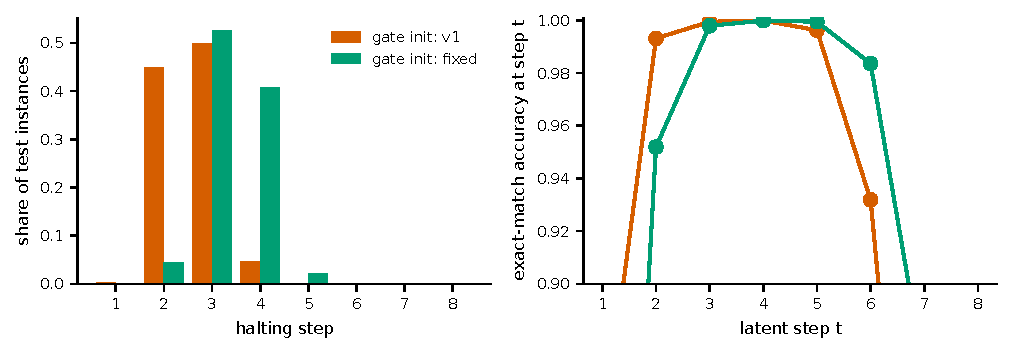
\includegraphics[width=\linewidth]{figures/figA_v1_corrected.pdf}
  \caption{v1 GLWM re-evaluated: halting steps (left) and exact-match accuracy at each latent step
  (right) for the two gate initialisations.}
  \label{fig:v1}
\end{figure}

\paragraph{Per-step accuracy of the backbones.} \Cref{fig:stepacc} shows exact-match accuracy at every
step for both objectives. On addition, accuracy on every split rises to its plateau and stays there:
once an answer is right it stays right. On parity, OOD-both accuracy peaks and then decays for both
objectives, so the stable oracle sits below 100\% and the backbone fails Gate G1.

\begin{figure}[h]
  \centering
  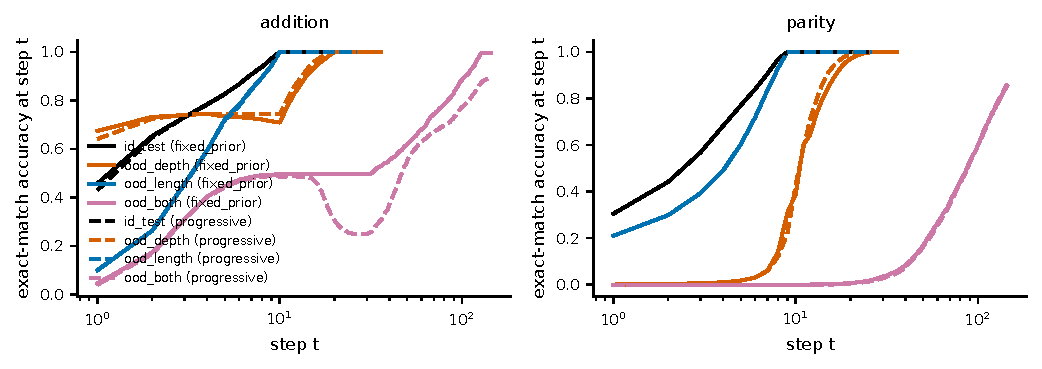
\includegraphics[width=\linewidth]{figures/figA_step_accuracy.pdf}
  \caption{Exact-match accuracy at step $t$ (mean over pilot seeds), fixed-prior (solid) and
  progressive (dashed) objectives.}
  \label{fig:stepacc}
\end{figure}

\begin{figure}[h]
  \centering
  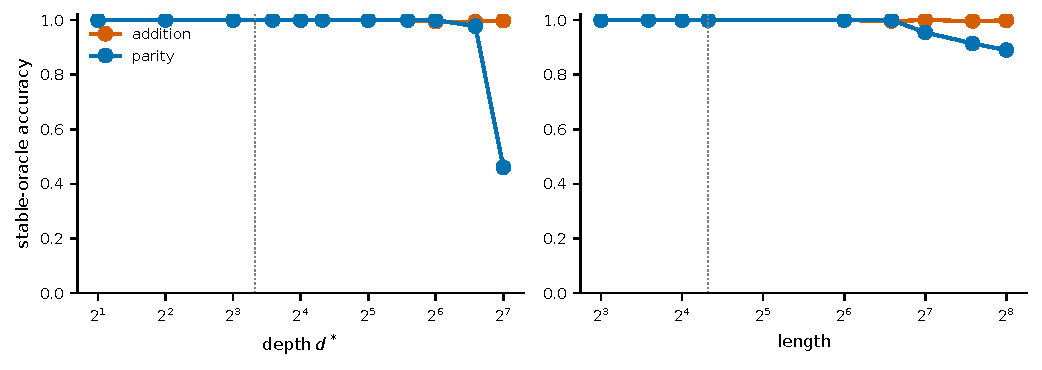
\includegraphics[width=\linewidth]{figures/fig3_oracle_vs_depth_length.pdf}
  \caption{Stable-oracle accuracy against depth (left) and length (right), pooled over splits; dotted
  lines mark the training maxima. Length alone costs nothing; accuracy on parity drops with depth.}
  \label{fig:oracle}
\end{figure}

\paragraph{Information travels at the light-cone speed.} \Cref{fig:posstep} shows, for one OOD-both
addition instance, which output positions are correct at which step, together with the per-position
lower bound $\rho_i$ from \cref{prop:oracles}. No position can be certified before its bound, and the
backbone's positions settle along a wave that follows it, travelling one position per step from each
stop. \Cref{fig:donespread} shows the done
probabilities of the two post-hoc completion heads on a deep instance: they switch on along the same
wave, after the bound.

\begin{figure}[h]
  \centering
  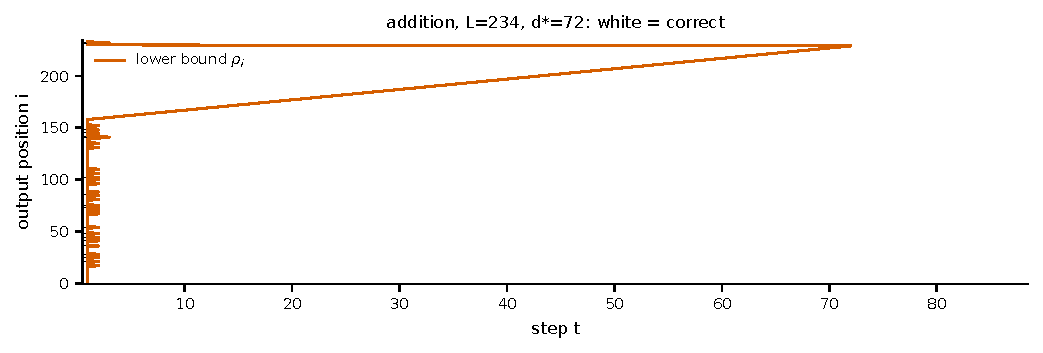
\includegraphics[width=\linewidth]{figures/figA_position_by_step.pdf}
  \caption{Correctness of every output position (rows) at every step (columns) for one OOD-both
  addition instance; white is correct. The orange line is the per-position lower bound $\rho_i$.}
  \label{fig:posstep}
\end{figure}

\begin{figure}[h]
  \centering
  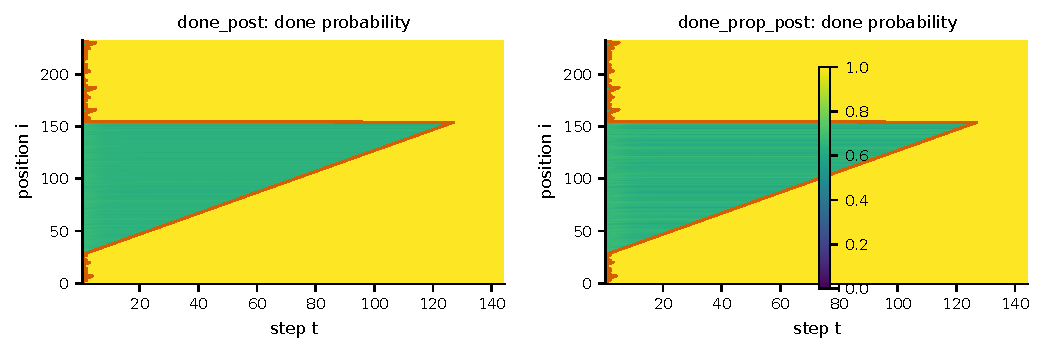
\includegraphics[width=\linewidth]{figures/figA_done_spread.pdf}
  \caption{Done probabilities of the post-hoc completion heads (pointwise, left; propagating, right) on a
  deep OOD-both addition instance, with the per-position lower bound in orange.}
  \label{fig:donespread}
\end{figure}

\paragraph{Linear probes.} A linear probe fitted on ID-val hidden states decodes whether a position is
still pending ($t < \rho_i$) from $h_i^{(t)}$, and transfers to OOD-depth and OOD-both without refitting
(\cref{tab:probes}). The backbone therefore represents the pending bit of the automaton in
\cref{prop:automaton}; whether a stopping rule uses it is a separate question.

\IfFileExists{tables/probes_ablations.tex}{\begin{table}[h]
\centering
\caption{Left: linear probe for the pending state (fitted on ID-val, seed-0 base model on addition). Middle: ablations on addition (seed 0; accuracy in \%). Right: CUDA-event latency for 512 OOD-depth instances with online early exit (median ms).}
\label{tab:probes}
\small
\begin{tabular}{lrr}
\toprule
Split & Acc. & AUC \\
\midrule
id-test & 100.0 & 1.000 \\
ood-depth & 100.0 & 1.000 \\
ood-both & 100.0 & 1.000 \\
\bottomrule
\end{tabular}\quad
\begin{tabular}{llrr}
\toprule
Ablation & Rule & OOD-depth & OOD-both \\
\midrule
main & max softmax & 100.0 & 99.8 \\
main & oracle stable & 100.0 & 99.6 \\
no recall & max softmax & 100.0 & 7.5 \\
no recall & oracle stable & 100.0 & 0.6 \\
r 2 & max softmax & 100.0 & 100.0 \\
r 2 & oracle stable & 100.0 & 100.0 \\
width 64 & max softmax & 100.0 & 48.0 \\
width 64 & oracle stable & 100.0 & 95.2 \\
\bottomrule
\end{tabular}\quad
\begin{tabular}{lr}
\toprule
Rule & ms \\
\midrule
fixed T (val-selected) & 7.4 \\
fixed T = T max & 23.8 \\
max softmax & 19.8 \\
done post & 23.8 \\
done prop post & 28.3 \\
\bottomrule
\end{tabular}
\end{table}
}{}

\paragraph{Measured compute.} \Cref{fig:compute} plots measured FLOPs per instance (from
\texttt{FlopCounterMode}, at the mean length of each split) against accuracy. The completion heads add
one small MLP per position and step; their cost is dominated by the number of steps they choose.

\begin{figure}[h]
  \centering
  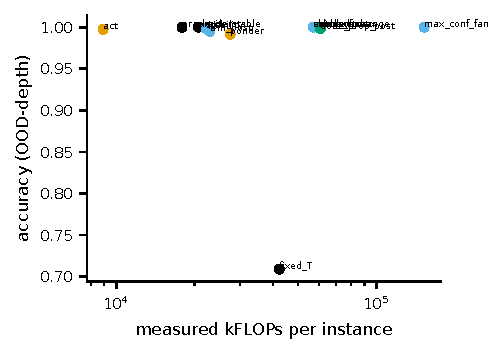
\includegraphics[width=0.6\linewidth]{figures/fig8_compute.pdf}
  \caption{Accuracy on addition OOD-depth against measured kFLOPs per instance for every stopping rule.}
  \label{fig:compute}
\end{figure}
